\documentclass[10pt,a4paper]{article}
\usepackage[margin=2.2cm]{geometry}
\usepackage{amsmath,amssymb,amsfonts,mathtools}
\usepackage{booktabs,tabularx,longtable,array,multirow}
\usepackage{graphicx}
\usepackage[dvipsnames]{xcolor}
\usepackage{hyperref}
\usepackage{listings}
\usepackage{enumitem}
\usepackage{tikz}
\usetikzlibrary{arrows.meta,positioning,shapes.geometric,fit}
\usepackage{caption}
\usepackage{subcaption}
\usepackage{float}
\usepackage{fancyhdr}
\hypersetup{colorlinks=true,linkcolor=NavyBlue,urlcolor=NavyBlue,citecolor=NavyBlue}
\setlist{itemsep=2pt,topsep=3pt}
\lstset{basicstyle=\ttfamily\footnotesize,breaklines=true,frame=single,framesep=3pt,columns=fullflexible,
  backgroundcolor=\color{gray!6},rulecolor=\color{gray!40},showstringspaces=false}
\newcommand{\code}[1]{\texttt{#1}}
\newcommand{\R}{\mathbb{R}}
\newcommand{\E}{\mathbb{E}}
\newcommand{\1}{\mathbb{1}}
\newcommand{\insight}[1]{\par\smallskip\noindent\colorbox{NavyBlue!7}{\parbox{\dimexpr\linewidth-2\fboxsep}{\small\textbf{Intuition.} #1}}\par\smallskip}
\newcommand{\finding}[1]{\par\smallskip\noindent\colorbox{ForestGreen!8}{\parbox{\dimexpr\linewidth-2\fboxsep}{\small\textbf{Finding.} #1}}\par\smallskip}
\pagestyle{fancy}\fancyhf{}\rhead{\small Gemma-RL technical report}\lhead{\small 2 Oct 2026}\cfoot{\thepage}
\setlength{\headheight}{12pt}

\title{\textbf{Gemma-RL: Technical Report}\\[4pt]
\large Building a Gemma-4-31B software-engineering agent for the Kaggle \emph{Gemma 4 Developer Agent}
competition, and researching learned (RL) graph traversal for fault localization}
\author{Project team \quad (prepared with Claude Code)}
\date{Status as of 2 October 2026}

\sloppy
\begin{document}
\maketitle
\begin{abstract}
\noindent This report documents everything done so far in the Gemma-RL project: the problem and its
constraints, the data, the evaluation infrastructure we had to build (a Docker-free reproduction of the
official harness, model serving on two shared 24\,GB GPUs with a patched vLLM, and a Kaggle evaluation
pipeline on the scorer's real hardware), the fault-localization research (ground-truth labelling,
BM25 / embedding / learning-to-rank baselines under leave-one-repository-out validation, graph smoothing,
and a deployed BM25 locator skill), eight end-to-end agent configurations (C1--C6) evaluated on the
scorer hardware with failure triage, the measurement protocol, the groundwork for fine-tuning (LoRA
loading, exact-format supervised data rendering, compaction-aware dataset construction), new training
data (66 verified tasks mined from git history, 1{,}628 synthetic localization bugs with LLM-written issues),
and the formal design of the reinforcement-learning traverser. Every number in this report comes from
files in the repository; the methodology is given with both intuition and the underlying mathematics.
\end{abstract}

\tableofcontents
\newpage

%==========================================================================================
\section{Executive summary}
\begin{table}[H]\centering\small
\begin{tabularx}{\linewidth}{>{\raggedright\arraybackslash}p{4.2cm}X}
\toprule
\textbf{Area} & \textbf{Result} \\ \midrule
Competition & 129 public tasks (fastapi 67, rich 48, requests 13, httpx 1); hidden set $\approx$120 tasks; 12\,h runtime; 1 submission/day; model fixed to \code{gemma-4-31b-it-qat-w4a16-ct}. \\
Local harness & Docker-free, faithful to the scorer's verification; \textbf{107/129} tasks are locally \emph{valid} (gold patch passes, empty patch fails). \\
Serving & 31B W4A16 model served on 2 shared A5000s via an uneven pipeline split (52/8 layers), 4 vLLM patches, $\approx$21.5 tok/s per stream. \\
Localization (LORO) & BM25 node MRR \textbf{0.398}; supervised LambdaMART ranker 0.397$\pm$0.012; graph smoothing 0.385; embedding pseudo-query 0.112. With 3 training repositories the learned ranker does \emph{not} beat BM25. \\
Locator skill & File hit@1 \textbf{0.49}, hit@3 0.69 (public best known: 0.43 / 0.70@5), $<$1\,s per call. \\
Agent (scorer HW, same 30 tasks) & Best configurations solve 9--10/30 (30--33\%); per-run std $\approx$0.024; 8 runs jointly solve \textbf{14/30}: pass@8 = 0.467 vs pass@1 = 0.29. \\
Key failure modes fixed & malformed skill calls (backticks), test-file edits that break hidden-test application (0 after fix), thinking-driven timeouts, empty submissions under tight tool budgets. \\
Submissions & C4 submitted (pending); C6a (same accuracy, 34\% faster) frozen as \code{scaffold-v1-frozen}, next submission. \\
Fine-tuning groundwork & LoRA (rank 16, 122M params, 233.5\,MiB) loads on the QAT checkpoint and changes outputs; SFT rendering reproduces vLLM's prompts token-exactly on 15/16 turns. \\
New data & 66 verified mined tasks; 1{,}628 injected bugs in 22 packages; own graph builder with node parity 1.00 on non-test code. \\
\bottomrule
\end{tabularx}
\caption{One-page summary of results.}
\end{table}

\insight{The model already \emph{can} solve far more tasks than it solves in any single attempt
(pass@8 $\gg$ pass@1). That gap is the central quantitative fact of the project so far: it makes
rejection-sampling fine-tuning (train on the model's own successes) the main competition lever, while
better localization matters less than expected because most failures are ``right file, wrong fix''.}

%==========================================================================================
\section{Problem setting}
\subsection{The task}
Each task $t$ is a real GitHub pull request from one of four Python repositories, given as the tuple
\[(\text{repo},\ \text{base commit},\ \text{problem statement},\ \text{hints},\ \text{gold patch } p^\star,\ \text{test patch}).\]
The agent sees only the repository at \code{base\_commit} and the problem statement (hints are empty for
all 129 public tasks). It must produce a patch $p$. Scoring happens in a fresh sandbox: apply $p$, reset
any test/config files, apply the hidden \code{test\_patch}, run \code{pytest} on the targeted test files.
\begin{align*}
R(t,p)&=\1\big[\text{pytest exits }0\ \wedge\ \text{passed}>0\ \wedge\ \text{failures}=\text{errors}=0\ \wedge\ \text{all required tests passed}\big],\\
\text{Score}&=\frac{1}{|T|}\sum_{t\in T}R(t,p_t).
\end{align*}
\subsection{Constraints that shaped every decision}
\begin{itemize}
\item \textbf{Fixed model:} all agents must use \code{gemma-4-31b-it-qat-w4a16-ct} (31B parameters, weights quantized to 4\,bit with group size 32, activations 16\,bit), served by vLLM with tensor parallelism 4 on 4$\times$L4 (24\,GB each), \code{max\_model\_len}=32{,}768, \code{gpu\_memory\_utilization}=0.80.
\item \textbf{Declarative submissions only:} \code{agent.yaml}, prompts, sampling config, optional LoRA adapters (\code{.safetensors}), and ADK \emph{skills} (\code{SKILL.md} + Python scripts). No arbitrary Python entrypoint; allowed file types \code{.yaml .yml .md .txt .py .json .safetensors}; $<$3\,GiB.
\item \textbf{Budgets:} per-task time / tool calls / turns from \code{eval\_config.yaml}; ADK compacts the conversation once it exceeds 14{,}336 tokens.
\item \textbf{Runtime:} $\approx$120 hidden tasks in 12 hours; if tasks run serially that is $\le$6 minutes per task on average.
\item \textbf{Rules} (\code{reports/rules.md}): external data allowed if public and free; open-source code must be OSI-licensed without commercial restrictions; winners release code (Apache-2.0); 1 submission/day, 2 final selections; no private sharing outside the team.
\end{itemize}

%==========================================================================================
\section{Data}
\subsection{Audit}
\begin{table}[H]\centering\small
\begin{tabular}{lrrrrrr}\toprule
repo & tasks & median graph nodes & median files & median hunks & median +lines & median $-$lines\\\midrule
fastapi & 67 & 3931 & 1 & 2 & 11 & 2\\
rich & 48 & 1970 & 1 & 2 & 5 & 3\\
requests & 13 & 733 & 1 & 1 & 3 & 1\\
httpx & 1 & 740 & 7 & 18 & 57 & 22\\\bottomrule
\end{tabular}\caption{Data audit (\code{src/dataio/audit.py}). Gold patches are small and never touch tests.}
\end{table}
\begin{figure}[H]\centering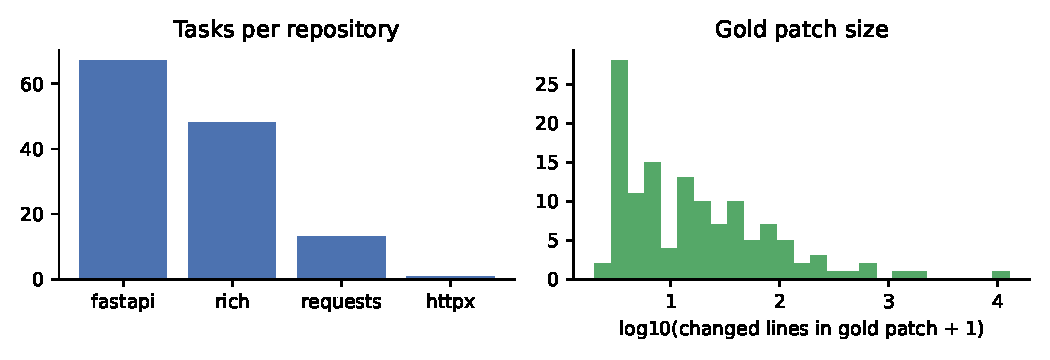
\includegraphics[width=0.85\linewidth]{figs/audit.pdf}\caption{Tasks per repository and gold-patch size distribution.}\end{figure}
Each task ships a code graph (JSON, one per base commit) and node embeddings (256-dimensional, unknown
encoder). Graph nodes are $\{\code{id},\code{name},\code{text}\}$ with dotted names such as
\code{requests.utils.get\_encoding\_from\_headers}; there is a single edge type \code{calls} which, as we
discovered while building our own graph (\S\ref{sec:graphbuild}), stores every relation in \emph{both}
directions and also encodes class$\leftrightarrow$method containment. Nodes carry no file paths or line numbers.

\insight{With one repository dominating (fastapi 52\%) and httpx contributing a single task,
leave-one-repository-out (LORO) validation effectively has three folds. Any learned component sees only
two or three repositories during training --- the root cause of several later findings.}

%==========================================================================================
\section{Infrastructure}
\subsection{Three Python environments}
The harness wheels target CPython 3.12 (vLLM, torch 2.10/CUDA 12.8), while the scorer's sandbox image is
\code{python:3.13-slim}. We therefore keep: \code{.venv} (3.13, research code), \code{.venv-harness}
(3.12, model server only) and \code{.venv-eval} (3.13 on a clean standalone interpreter, harness without
torch). The sandbox inherits the interpreter's site-packages, so a clean base interpreter is essential
--- the system Python carried 706 Debian packages that would have leaked into the sandbox.

\subsection{A Docker-free reproduction of the scorer}
No container runtime exists on the server, so evaluation uses the harness's subprocess sandbox. Out of the
box it skips dependency installation (on Kaggle the notebook image already has everything). We patched it
(\code{src/eval/harness\_patches.py}) to resolve each task's dependencies with \code{pip} from the offline
wheel directory \emph{under the repository's own version constraints}. Installing the newest version of
every wheel (what the Docker path does) shadows the repository's own package and breaks older commits
(e.g.\ \code{starlette 1.6} removed \code{on\_startup}). We reconstructed the scorer image's test-only
plugins from evidence in the harness (\code{pytest-httpbin}, \code{inline-snapshot}, \code{dirty-equals}, \dots).

\paragraph{Validity.} A task is \emph{locally valid} iff the gold patch resolves it and an empty patch does not:
\[
V=\{t:\ R(t,p^\star_t)=1\ \wedge\ R(t,\varnothing)=0\}.
\]
\begin{table}[H]\centering\small
\begin{tabular}{lrrl}\toprule
repo & valid & total & main reasons for exclusion \\\midrule
fastapi & 58 & 67 & dependency drift; 2 tasks pass with an empty patch\\
rich & 39 & 48 & newer pygments / markdown-it change rendered output\\
requests & 9 & 13 & idna validation drift, one SSL-certificate failure\\
httpx & 1 & 1 & -- \\\midrule
total & \textbf{107} & 129 & \\\bottomrule
\end{tabular}\caption{Local validity (\code{data/derived/valid\_tasks.txt}).}
\end{table}

\subsection{Serving a 31B model on two shared 24\,GB GPUs}
\paragraph{Memory arithmetic.} One decoder layer has attention projections $q: 5376\!\to\!8192$,
$k,v: 5376\!\to\!4096$, $o: 8192\!\to\!5376$ (sliding-window layers) and an MLP of three
$5376\leftrightarrow21504$ matrices:
\[
P_\text{layer}\approx 44.0\text{M}+2\cdot22.0\text{M}+44.0\text{M}+3\cdot115.6\text{M}\approx 479\text{M parameters}.
\]
W4A16 with group size 32 stores 4 bits per weight plus a 16-bit scale per 32 weights,
i.e.\ $0.5+2/32=0.5625$ bytes/parameter, so $\approx 269$\,MB $\approx 0.25$\,GiB per layer --- matching the
measured 0.27\,GiB/layer (16.58\,GiB for 53 layers + embedding vs 16.86\,GiB for 54). The embedding is
$262{,}144\times5{,}376$ in bf16 $=2.62$\,GiB, and with pipeline parallelism the last stage needs its own copy of the
tied output head. Tensor parallelism over two GPUs needs $\approx$12\,GiB of weights per GPU plus KV cache;
the second GPU never had more than 9.2\,GiB free (another user's server holds 15\,GiB).

\paragraph{KV cache.} Gemma-4-31B is hybrid: 50 sliding-window layers (window 1024) and 10 global layers
(4 KV heads, head dim 512). The KV bytes per token of context come almost entirely from global layers:
$10\times4\times512\times2\,(\text{K},\text{V})\times2\,\text{bytes}=80$\,KiB. vLLM's measured requirement for one
full-length request fits a line
\[
\text{KV}(L)\approx a+bL,\qquad b\approx 70\ \text{KiB/token},\ a\approx2.2\ \text{GiB}
\]
from the points $(20{,}480,3.55)$, $(24{,}576,3.81)$, $(32{,}768,4.37)$ GiB --- $b$ is consistent with the 80\,KiB
estimate; $a$ is the fixed sliding-window/prefill-chunk allocation.

\paragraph{Solution: an uneven pipeline split.} Pipeline parallelism (PP=2) with \code{VLLM\_PP\_LAYER\_PARTITION=52,8}
places 52 layers on GPU0 and 8 layers + output head on GPU1. Four local patches to vLLM were needed
(\code{scripts/patch\_vllm\_gemma4\_pp.py}):
\begin{enumerate}
\item Gemma-4's PP path called \code{IntermediateTensors.get()} (no such method) and sent \code{None}
  residual/per-layer tensors between stages. Each layer ignores its incoming residual, so sending zeros is
  numerically identical.
\item A per-rank KV budget (\code{GEMMA\_RL\_KV\_GIB\_PER\_RANK}), because one global budget cannot fit both
  an almost-full and an almost-empty GPU.
\item Clamping \code{max\_tokens} to the remaining context instead of rejecting requests (the scorer's 32k
  context leaves room that our 20k context does not).
\end{enumerate}
plus the Kaggle-wheelhouse vLLM build (PyPI's build lacks LoRA support for Gemma-4), FastAPI $<$0.130,
and \code{--reasoning-config} with Gemma's channel tokens. Concurrency $>$1 triggered a PP scheduler stall
after preemption, so the server runs one sequence at a time (\code{MAX\_SEQS=1}). Throughput: 21.5
tokens/s per stream. The working configuration is \code{scripts/start\_server.sh}.

\subsection{Evaluation on the scorer's hardware}
Kaggle notebooks run on the same 4$\times$L4 machine type as the scorer. \code{scripts/kaggle\_eval/} builds a
private kernel per experiment: it installs the official wheelhouse exactly like the organizers' starter
notebook, serves the model with the scorer's vLLM settings, runs the official \code{Evaluator} with the
scorer's compaction settings (interval 5, overlap 2, threshold 14{,}336, retention 5) at concurrency 4, and
downloads results, patches, test logs and full traces. Two fixes were required: a private dataset with the
test-only packages the Kaggle image lacks (without it every fastapi test fails on \code{inline\_snapshot}),
and an in-kernel \emph{capture proxy} that records every LLM request/response for supervised training data.

%==========================================================================================
\section{Fault localization research}
\label{sec:loc}
\subsection{Ground-truth labels from gold patches (B1)}
Localization has free supervision. For a gold patch, let $\mathcal L$ be the changed old-file line numbers
(removed lines, and for pure insertions the line above the insertion point). Parsing the file at
\code{base\_commit} with Python's \code{ast} yields the qualified-name spans
$\{(q,\ell_\text{start},\ell_\text{end})\}$ of all definitions (decorators included). The module prefix $m$ of a file
is the dotted suffix of its path that maximizes the number of definitions found in the graph. A changed line
$\ell$ maps to the innermost span containing it whose name $m.q$ exists in the graph:
\[
\text{target}(\ell)=\arg\min_{(q,s,e):\ s\le \ell\le e,\ m.q\in G}\ (e-s).
\]
Results: 117/129 tasks (91\%) have $\ge$1 target node; unmapped lines are mostly module-level (imports,
constants: 1{,}127) or functions missing from the provided graph (92).
\begin{figure}[H]\centering
\begin{subfigure}{0.48\linewidth}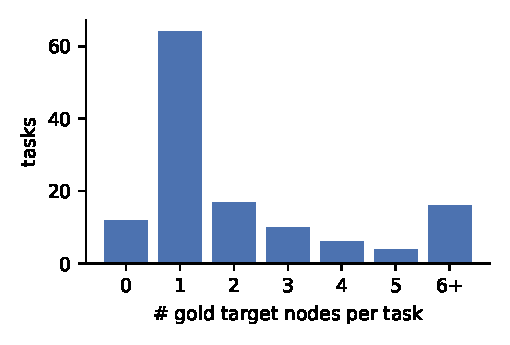
\includegraphics[width=\linewidth]{figs/b1_targets.pdf}\caption{Gold nodes per task.}\end{subfigure}
\begin{subfigure}{0.48\linewidth}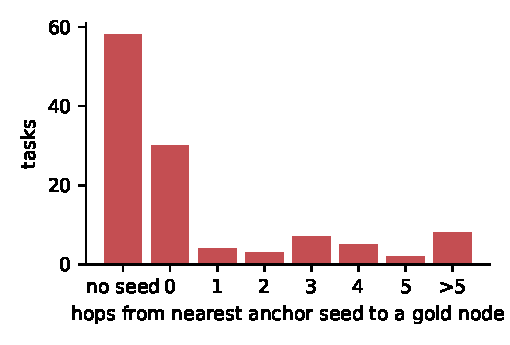
\includegraphics[width=\linewidth]{figs/seed_dist.pdf}\caption{Graph distance from issue anchors to gold.}\end{subfigure}
\caption{Label statistics. (b) For 58 of 117 tasks no issue identifier selects a specific node (anchor
matches $>$25 nodes or none); for 30 an anchor hits a gold node directly; the rest need 1--5 hops.}
\end{figure}
\insight{Half the issues contain no selective identifier, so any graph traversal must start from lexical
retrieval (BM25) rather than from names in the issue; and when a name is present, it is very often the
answer itself (distance 0). The remaining tasks, where the answer is a few hops from a named symbol, are
exactly where learned traversal could help.}

\subsection{Anchors}
From the issue text we extract: identifiers inside backticks; snake\_case / CamelCase / dotted tokens; file
paths; traceback frames. An anchor's weight is its inverse document frequency over node short names,
$w(a)=\log(1+N/n_a)$ where $n_a$ is the number of nodes with that short name; anchors matching $\le$25 nodes
become graph \emph{seeds}.

\subsection{R1: BM25}
Nodes are documents $d$ whose tokens are the name tokens (camel/snake-split, weighted $\times$3) plus the
tokenized source text. For query tokens $q$:
\[
\text{BM25}(d,q)=\sum_{w\in q}\text{idf}(w)\,\frac{f(w,d)\,(k_1+1)}{f(w,d)+k_1\big(1-b+b\,\frac{|d|}{\text{avgdl}}\big)}\cdot\min(\text{qtf}_w,3),
\qquad \text{idf}(w)=\log\Big(1+\frac{N-n_w+0.5}{n_w+0.5}\Big),
\]
with $k_1=1.2$, $b=0.75$. \emph{Intuition:} term frequency saturates (a word appearing 20 times is not 20$\times$
more relevant), rare words count more, long nodes are normalized.

\subsection{R2: embedding pseudo-query}
The 256-d node embeddings come from an unknown encoder, so the issue cannot be embedded. We form a
pseudo-query from the seeds $S$ (or BM25's top-5 when there are none):
$\mathbf c=\frac{\sum_{i\in S}\mathbf e_i}{\|\sum_{i\in S}\mathbf e_i\|}$ and score $s_i=\mathbf e_i^\top\mathbf c$ (embeddings
$\ell_2$-normalized). This mirrors the harness tool \code{search\_similar\_code}, which also only accepts symbol names.

\subsection{R3: learning to rank (LambdaMART)}
Every non-test node gets a 29-dimensional feature vector: BM25 (raw, max-normalized, rank percentile,
name-only), embedding cosine/rank/max-to-seed, anchor matches (idf-weighted short name, backtick,
dotted-path, traceback, mentioned module, parent/child anchors), graph distance to seeds and to BM25's
top-5, degree, node kind, privacy/dunder flags, depth, in-package flag, text length, name--query overlap and
the best BM25 score in the same module. LightGBM's LambdaRank optimizes NDCG directly: for a pair
$(i,j)$ with $y_i>y_j$ in the same query, the gradient on $s_i$ is
\[
\lambda_{ij}=\frac{-\sigma}{1+e^{\sigma(s_i-s_j)}}\;\big|\Delta\text{NDCG}_{ij}\big|,\qquad
\lambda_i=\sum_{j:y_i>y_j}\lambda_{ij}-\sum_{j:y_j>y_i}\lambda_{ji},
\]
i.e.\ a RankNet pairwise logistic gradient re-weighted by how much swapping $i$ and $j$ would change NDCG.
Training uses all positives plus hard negatives (top-100 by BM25, embedding and anchor score) and 200
random negatives per task; 300 rounds, 15 leaves, learning rate 0.05, 3 seeds; folds are LORO.

\subsection{R3+G: graph smoothing}
With $z_i$ the per-task z-scored ranker output and $\mathcal N(i)$ the undirected neighbours,
\[
s'_i=z_i+\alpha\max_{j\in\mathcal N(i)} z_j ,
\]
with $\alpha\in\{0,0.1,\dots,0.75\}$ chosen per fold on the \emph{other} folds' out-of-fold predictions.

\subsection{Metrics}
For a ranking $\pi$ of candidates and gold set $T$:
$\text{Recall@}k=\frac{|\pi_{1..k}\cap T|}{|T|}$, $\text{Hit@}k=\1[\pi_{1..k}\cap T\neq\varnothing]$,
$\text{MRR}=1/\text{rank of the first gold}$, $\text{nDCG@10}=\frac{\sum_{r\le10,\pi_r\in T}1/\log_2(r+1)}{\sum_{r=1}^{\min(|T|,10)}1/\log_2(r+1)}$.
File-level Hit@$k$ deduplicates the node ranking into a module ranking.

\subsection{Results}
\begin{table}[H]\centering\footnotesize\setlength{\tabcolsep}{3.5pt}
\begin{tabular}{llrrrrrrr}\toprule
fold & system & R@1 & R@5 & R@10 & Hit@5 & MRR & nDCG@10 & File@1\\\midrule
\multirow{4}{*}{ALL (117)} & R1 BM25 & .183 & .384 & .457 & .513 & \textbf{.398} & \textbf{.373} & .496\\
 & R2 embedding & .047 & .099 & .116 & .154 & .112 & .091 & .248\\
 & R3 ranker & .185 & .369 & .444 & .501 & .397 & .358 & \textbf{.501}\\
 & R3+G & .177 & .373 & .432 & .501 & .385 & .350 & .487\\\midrule
fastapi (60) & R1 / R3 & .163/.136 & .354/.303 & .448/.368 & .483/.428 & \textbf{.390}/.331 & .371/.305 & .433/.367\\
rich (45) & R1 / R3 & .148/.164 & .332/.363 & .387/.462 & .467/.511 & .358/\textbf{.412} & .305/.354 & .533/.615\\
requests (11) & R1 / R3 & .455/.545 & .788/.778 & .818/.818 & .818/.818 & .616/\textbf{.643} & .663/.681 & .636/.727\\\bottomrule
\end{tabular}\caption{LORO localization (\code{reports/localization\_baselines.md}); R3 values are means over 3 seeds (std $\le$0.04).}
\end{table}
\begin{figure}[H]\centering
\begin{subfigure}{0.6\linewidth}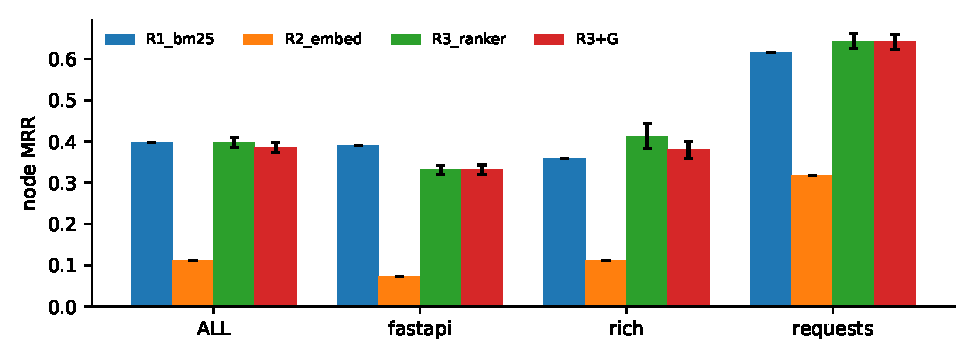
\includegraphics[width=\linewidth]{figs/b2_mrr.pdf}\caption{Node MRR per fold.}\end{subfigure}
\begin{subfigure}{0.38\linewidth}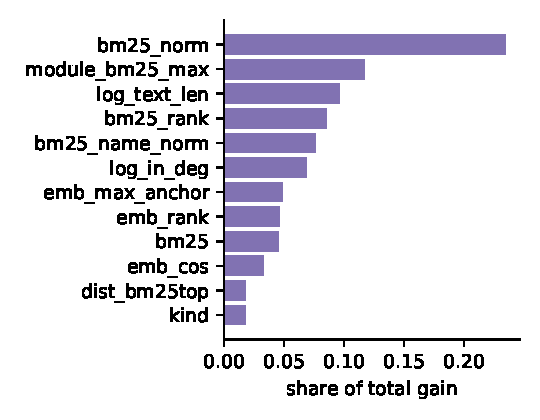
\includegraphics[width=\linewidth]{figs/b2_importance.pdf}\caption{R3 feature importance (gain).}\end{subfigure}
\caption{Localization baselines.}\end{figure}
\finding{BM25 is the baseline to beat. The supervised ranker matches it overall, wins on rich and requests,
and loses on fastapi when trained on only two other repositories; its most important features are
themselves lexical. Graph smoothing does not help. The bottleneck is \emph{training data}, not model
capacity --- which motivates the mined and synthetic data of \S\ref{sec:data}.}

\subsection{The deployed locator skill}
\code{skills/repo-tools/scripts/locate.py} (pure standard library, runs inside the sandbox) parses every
non-test Python file with \code{ast}, scores each definition with BM25 over name tokens ($\times$3) + body (first
120 lines) + path tokens, then adds anchor bonuses
\[
s_i=\frac{\text{BM25}_i}{\max_j\text{BM25}_j}+\underbrace{\tfrac{0.6}{\sqrt{c_i}}\1[\text{backtick}]}_{\text{or }0.3\text{ for identifiers}}
+0.4\,\1[\text{dotted match}]+0.25\,\1[\text{file mentioned}]+\lambda_\text{path}\,\frac{\sum_{w\in P_i\cap q}\text{idf}_f(w)}{\sum_{w\in P_i}\text{idf}_f(w)},
\]
where $c_i$ counts definitions sharing the short name and $P_i$ are the tokens of the file path
(generic tokens such as \code{utils} removed), with idf computed over files. The last term captures
concept-to-file mappings (``OpenAPI'' $\to$ \code{openapi/utils.py}).
\begin{figure}[H]\centering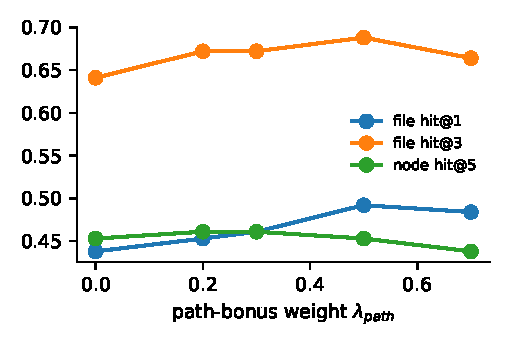
\includegraphics[width=0.45\linewidth]{figs/locate_sweep.pdf}
\caption{Sweep of $\lambda_\text{path}$ on 128 tasks; $\lambda_\text{path}=0.5$ is used (file hit@1 0.438$\to$0.492, hit@3 0.641$\to$0.688).}\end{figure}

%==========================================================================================
\section{The agent (scaffold) and end-to-end experiments}
\subsection{How the harness drives an agent}
\begin{figure}[H]\centering
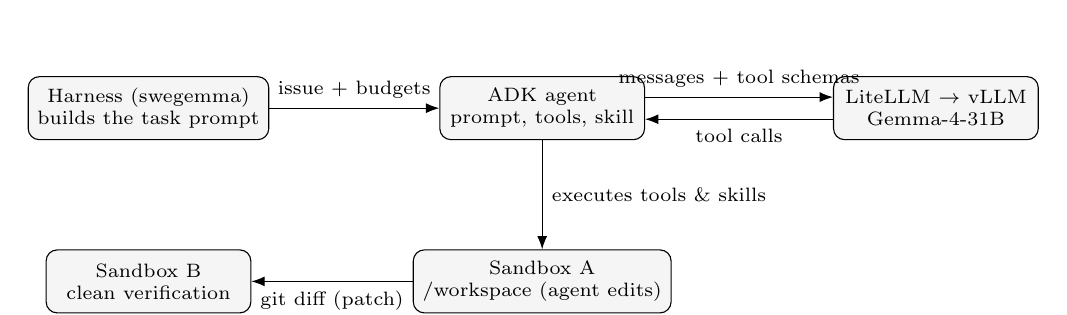
\begin{tikzpicture}[every node/.style={font=\scriptsize}, box/.style={draw,rounded corners,fill=gray!8,align=center,minimum height=0.8cm,minimum width=2.6cm}]
\node[box] (h) at (0,0) {Harness (swegemma)\\builds the task prompt};
\node[box] (a) at (5,0) {ADK agent\\prompt, tools, skill};
\node[box] (l) at (10,0) {LiteLLM $\to$ vLLM\\Gemma-4-31B};
\node[box] (s) at (5,-2.2) {Sandbox A\\/workspace (agent edits)};
\node[box] (v) at (0,-2.2) {Sandbox B\\clean verification};
\draw[-{Latex}] (h) -- node[above]{issue + budgets} (a);
\draw[-{Latex}] ([yshift=4pt]a.east) -- node[above]{messages + tool schemas} ([yshift=4pt]l.west);
\draw[-{Latex}] ([yshift=-4pt]l.west) -- node[below]{tool calls} ([yshift=-4pt]a.east);
\draw[-{Latex}] (a) -- node[right]{executes tools \& skills} (s);
\draw[-{Latex}] (s) -- node[below]{git diff (patch)} (v);
\end{tikzpicture}
\caption{Phase 1 runs the agent in sandbox A until \code{submit\_patch}, a budget limit or 3 nudges; phase 2 verifies the diff in a clean sandbox B.}\end{figure}
Tools: \code{run\_command}, \code{read\_file} (150 lines / 10k chars), \code{edit\_file} (3-tier fuzzy
replacement), \code{write\_file}, \code{get\_status}, \code{submit\_patch}, three graph tools, and the ADK skill
tools (\code{list\_skills}, \code{load\_skill}, \code{run\_skill\_script}). Skill calls do not count against the
tool budget. Our \code{repo-tools} skill provides \code{locate.py}, \code{show.py} (definition with line
numbers), \code{tests.py} (tests mentioning a name) and \code{check.py} (clean-up + compile + targeted pytest).

\subsection{Configurations}
\begin{table}[H]\centering\small
\begin{tabularx}{\linewidth}{lX}\toprule
C1 & Structured six-step prompt (anchors $\to$ locate $\to$ read $\to$ edit $\to$ verify $\to$ submit), repo-tools skill, thinking budget 2048, 8\,min / 45 tool calls. \\
C2 & + explicit tool list, JSON skill-call templates, ``edit by the 10th call'' rule. \\
C3 & Skill instructions as plain text (no backticks), fixed argument order. \\
C4 & + \code{check.py} automatically reverts test/config edits and deletes scratch files; time rule. \\
C5a / C5b & C4 with thinking budget 1024 / thinking disabled. \\
C6a & Thinking disabled, 100 tool calls / 150 turns, ``never submit an empty patch''. \textbf{Frozen.} \\
C6b & Thinking 512, 80 tool calls, same rules. \\\bottomrule
\end{tabularx}\caption{Scaffold versions (\code{submissions/}).}\end{table}

\subsection{Results on the scorer's hardware}
All configurations were run on the same 30 locally valid tasks on Kaggle 4$\times$L4 with the scorer's settings.
\begin{table}[H]\centering\footnotesize\setlength{\tabcolsep}{4pt}
\begin{tabular}{lrrrrrrr}\toprule
config & resolved & mean s/task & timeouts & test-patch failures & right file, wrong fix & wrong location & no patch\\\midrule
C1 & 8 & 415 & 16 & 3 & 10 & 5 & 1\\
C2 & 8 & 415 & 13 & 4 & 10 & 4 & 0\\
C3 & \textbf{10} & 428 & 14 & 1 & 11 & 3 & 1\\
C4 & 9 & 409 & 17 & \textbf{0} & 8 & 3 & 0\\
C5a & 9 & 401 & 14 & 0 & 11 & 3 & 1\\
C5b & 7 & \textbf{186} & 2 & 1 & 6 & 2 & 13\\
C6a & 9 & 270 & 4 & 1 & 6 & 3 & 7\\
C6b & 9 & 420 & 16 & 0 & 10 & 2 & 0\\\bottomrule
\end{tabular}\caption{End-to-end results (\code{reports/triage\_*.md}). ``Timeouts'' counts sessions stopped by the time budget (their partial patch is still scored).}\end{table}
\begin{figure}[H]\centering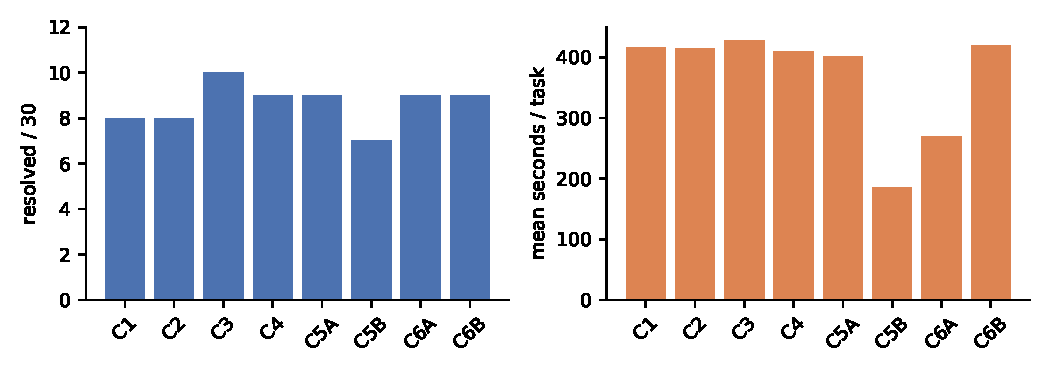
\includegraphics[width=0.85\linewidth]{figs/cseries.pdf}\caption{Resolved tasks and mean time per task.}\end{figure}

\subsection{Four failure mechanisms we found and fixed}
\paragraph{1. Malformed skill calls.} Gemma emits tool calls in a native syntax where string values are
delimited by a special token \code{<|"|>}. When the prompt showed paths inside markdown backticks, the model
sometimes closed a string with a backtick, producing \code{"file\_path": "scripts/locate.py`,skill\_name:"} and
losing the required argument (C2: 30 of 35 locate calls malformed). Writing all skill instructions as plain
text (C3) removed the problem.
\paragraph{2. The test-patch trap.} Verification resets protected test files and then applies the hidden
test patch. We reproduced locally that if the agent edited a test file that the hidden patch also touches,
the hidden patch fails to apply and the task scores 0 regardless of the fix (3--4 tasks per run in C1/C2).
\code{check.py} now reverts such edits automatically (0 failures in C4).
\paragraph{3. Thinking-driven timeouts.} Thinking volume and task duration correlate strongly ($r=0.72$,
Fig.~\ref{fig:think}); single thoughts reached the 2048-token cap, and at $\approx$20 tokens/s each such thought
costs $\approx$100\,s of an 8-minute budget.
\paragraph{4. Budget-bound empty submissions.} Without thinking the agent is 2.2$\times$ faster but makes
$\approx$40 shallow calls in $\approx$90\,s, hits the 45-call budget, and submits nothing (13/30 in C5b). C6a raises the
budget to 100 calls and forbids empty submissions: same accuracy as C4 at 66\% of the time.
\begin{figure}[H]\centering
\begin{subfigure}{0.48\linewidth}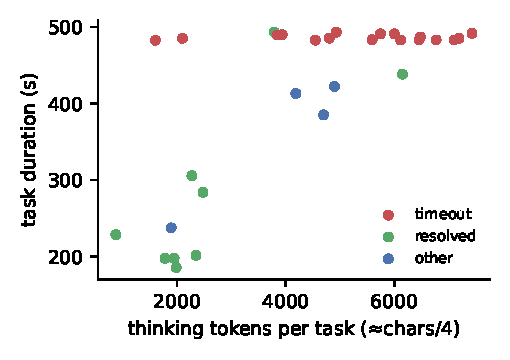
\includegraphics[width=\linewidth]{figs/thinking_time.pdf}\caption{C4: thinking vs duration.}\label{fig:think}\end{subfigure}
\begin{subfigure}{0.48\linewidth}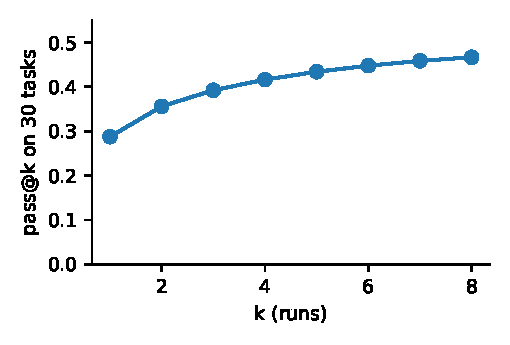
\includegraphics[width=\linewidth]{figs/passk.pdf}\caption{pass@$k$ across the 8 runs.}\end{subfigure}
\caption{Diagnostics.}\end{figure}

\subsection{How much of a difference is real? Noise, pass@k and stochastic tasks}
With per-task success probability $p\approx0.3$ and $n=30$ tasks the binomial standard error is
$\sqrt{p(1-p)/n}\approx0.084$, i.e.\ $\pm2.5$ tasks; with $n=107$ it is $0.044$ ($\pm$4.7 tasks). The observed run-to-run
standard deviation across configurations was 0.024. Differences of one or two tasks on 30 are therefore not
evidence. The plan's protocol (\S\ref{sec:protocol}) uses 107 tasks, $\ge$4 runs and paired tests.

Treating the 8 runs as samples, the unbiased pass@$k$ estimator is
\[
\text{pass@}k=\E_{t}\Big[1-\binom{n-c_t}{k}\Big/\binom{n}{k}\Big],
\]
where $c_t$ is the number of runs that solved $t$. It rises from 0.29 ($k{=}1$) to \textbf{0.467} ($k{=}8$): 14
distinct tasks are solvable; 4 are solved in all 8 runs (``stable'') and 10 only in some (``stochastic'').
\begin{figure}[H]\centering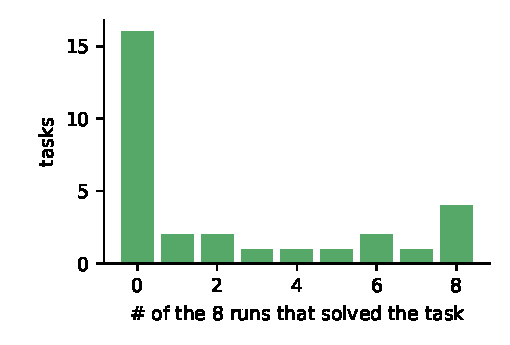
\includegraphics[width=0.45\linewidth]{figs/solve_freq.pdf}\caption{How many of the 8 runs solved each task.}\end{figure}
\insight{If the model were trained to make the choices it makes in its successful runs, single-run accuracy
should move from pass@1 towards pass@k. That is precisely what rejection-sampling fine-tuning does
(\S\ref{sec:sft}).}

%==========================================================================================
\section{Measurement protocol}
\label{sec:protocol}
Every competition-facing claim uses: the 107 valid tasks; $\ge$4 runs per configuration ($\ge$2 for the
organizers' sample baseline B0); pass@1 reported as mean$\pm$std across runs, pass@$k$, numbers of stable and
stochastic tasks, time per task, tool-error rate and tokens per task (\code{src/eval/scoreboard.py}). A difference
counts only if it exceeds twice the larger standard deviation or passes a paired test on per-task majority outcomes
(exact McNemar: with $b$ tasks only system A solves and $c$ only B,
$p=2\sum_{j=0}^{\min(b,c)}\binom{b+c}{j}2^{-(b+c)}$). Anything trained is evaluated LORO. Public-leaderboard scores
($\approx$60 tasks, 1 task $\approx$1.7\%) are never a selection criterion. On the pilot data (4 configurations, 30
tasks) the scoreboard gives pass@1 $0.300\pm0.024$, pass@4 0.467, 5 stable, 9 stochastic. The reference runs
(C6a$\times$4, B0$\times$2, 107 tasks) are queued on Kaggle.

%==========================================================================================
\section{Fine-tuning groundwork}
\label{sec:sft}
\subsection{LoRA on the quantized checkpoint}
LoRA adds a low-rank update to a frozen weight $W\in\R^{d_\text{out}\times d_\text{in}}$:
\[
h=Wx+\frac{\alpha}{r}BAx,\qquad A\in\R^{r\times d_\text{in}},\ B\in\R^{d_\text{out}\times r},
\]
so only $r(d_\text{in}+d_\text{out})$ parameters per matrix are trained, and the 4-bit base weights never change.
Gemma-4's global-attention layers have different shapes ($q: 5376\to16384$, $k: 5376\to2048$, no $v$ because
keys double as values), so adapter shapes are read from the checkpoint (\code{src/sft/make\_smoke\_adapter.py}).
For $r=16$ on all seven projections:
\[
50\times2.03\text{M}+10\times2.11\text{M}=122.4\text{M parameters}=233.5\ \text{MiB (bf16)},\quad 820\ \text{tensors}.
\]
The smoke test (random $A$, $B\sim\mathcal N(0,0.02^2)$) loads on the QAT checkpoint, and greedy outputs diverge
from the base model mid-sentence (``added functionality'' $\to$ ``enhanced functionality''), proving the adapter is
applied; decoding slows from 21.5 to 15 tokens/s locally (eager mode). The Kaggle-side test is queued.

\subsection{Supervised objective}
For a token sequence $x_{1:T}$ with loss mask $m_t\in\{0,1\}$ (1 exactly on tokens the model generated):
\[
\mathcal L(\theta)=-\frac{1}{\sum_t m_t}\sum_{t=1}^T m_t\log p_\theta(x_t\mid x_{<t}).
\]
Rejection-sampling fine-tuning (RFT/RAFT) samples $n$ trajectories per task at temperature 0.6--0.8, keeps those
whose patches pass the tests, and minimizes $\mathcal L$ on them. It is the special case of reward-weighted
regression with a binary reward: maximizing $\E_{\tau\sim\pi_\theta}[R(\tau)]$ by repeatedly fitting $\pi_\theta$ to the
reward-filtered distribution $\propto\pi_{\theta_\text{old}}(\tau)R(\tau)$. Expert iteration repeats this with the improved model.

\subsection{Rendering trajectories in the exact training format}
Training data is only useful if it matches, token for token, what the model sees at inference. We recorded the
real requests with a logging proxy and established:
\begin{itemize}
\item The system prompt is our instruction \emph{plus} ADK's agent-identity and skill-toolset text; the user message is the harness prompt; tool calls are assistant messages with JSON-string arguments; tool results are \code{tool} messages; 12 tool schemas.
\item vLLM parses argument strings into dicts before templating, producing Gemma's native call syntax:
\begin{lstlisting}
<|tool_call>call:read_file{end_line:650,filepath:<|"|>src/requests/models.py<|"|>,start_line:574}<tool_call|>
\end{lstlisting}
\item After tool calls the model stops by emitting the token \code{<|tool\_response>} (id 50); text answers end with \code{<turn|>} (id 106). Both are part of the training target.
\item With thinking disabled, the first generation of a model turn sees an empty thought channel that history renders never contain; we use the history format:
\begin{lstlisting}
<|channel>thought\n<channel|>
\end{lstlisting}
\end{itemize}
Round trip on a captured run: 15/16 of vLLM's prompts are exact token prefixes of our training sequence (the
16th differs only by those 3 empty-thought tokens), all 16 assistant spans are trained, and vLLM's own Gemma-4
tool parser recovers the original calls from the trained spans.

\subsection{Context compaction and segmentation}
ADK replaces old events with a summary once the context exceeds 14{,}336 tokens. 35 of 46 passing pilot
trajectories are longer than that (Fig.~\ref{fig:traj}), so the full trace is \emph{not} what the model saw.
The dataset builder (\code{src/sft/build\_dataset.py}) therefore uses the recorded per-call prompts: consecutive calls
belong to one \emph{segment} iff
\[
\text{prompt}_{k+1}[1{:}|\text{prompt}_k|+1]=\text{prompt}_k\ \Vert\ \text{response}_k ,
\]
and each segment becomes one sequence whose mask covers the assistant turns generated within it.
\begin{figure}[H]\centering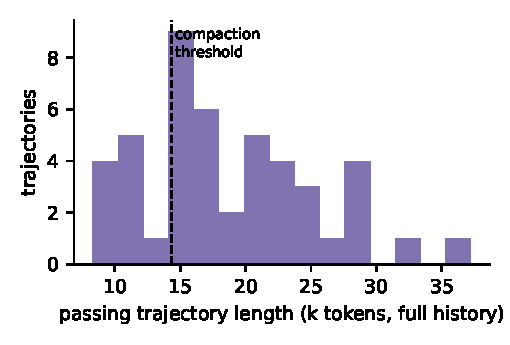
\includegraphics[width=0.45\linewidth]{figs/traj_len.pdf}\caption{Lengths of passing trajectories vs the compaction threshold.}\label{fig:traj}\end{figure}

%==========================================================================================
\section{New training data}
\label{sec:data}
\subsection{Tasks mined from git history (B4)}
Snapshots contain the full history before each base commit. A candidate is a non-merge commit touching both
source and test Python files, $\le$5 files and $\le$300 changed lines; its diff is split into \code{patch} (source) and
\code{test\_patch} (tests); the base is its parent; the commit message is the problem statement. \emph{Leakage
guard:} snapshot histories were rebuilt with \code{git fast-export}, so evaluation base SHAs are unresolvable; we keep
only commits older than the earliest evaluation PR minus 60 days and drop any commit whose hunks touch a function
changed by any evaluation gold patch.
\begin{table}[H]\centering\small
\begin{tabular}{lrrrl}\toprule
repo & commits before cutoff & candidates & verified & dominant failure\\\midrule
rich & 2902 & 260 & \textbf{62} & tests already pass without the fix (22)\\
fastapi & 5881 & 55 & 4 & 96\% of commits are docs/translations\\
requests & 4654 & 280 & 0 & \code{import cgi} (removed in Python 3.13), old urllib3\\\midrule
total & & 595 & \textbf{66} & \\\bottomrule
\end{tabular}\caption{Mining yield (\code{reports/b4\_mining.md}). 48/66 have short commit messages and will receive generated issue text.}\end{table}

\subsection{Our own code-graph builder}
\label{sec:graphbuild}
\code{src/graphbuild/build.py} reproduces the organizers' conventions: dotted names relative to the repository
root (\code{src/}, \code{docs\_src/} stripped, \code{\_\_init\_\_} collapsed); nested definitions named under the nearest
enclosing class or module; class text = header + docstring + method stubs; \code{calls} edges for containment and
for calls resolvable through imports or same-module definitions, stored in both directions.
\begin{table}[H]\centering\small
\begin{tabular}{lrrrr}\toprule
repo & node recall & node precision & edge recall & edge precision\\\midrule
fastapi & 1.000 & 0.828 & 0.731 & 0.644\\
rich & 1.000 & 0.999 & 0.919 & 0.950\\
httpx & 1.000 & 0.881 & 0.758 & 0.779\\
requests & 0.787$^\dagger$ & 0.787 & 0.695 & 0.733\\\bottomrule
\end{tabular}\caption{Parity with the provided graphs. $^\dagger$All requests mismatches are test-class members named differently; non-test parity is 1.0.}\end{table}

\subsection{Synthetic localization bugs (B5)}
From 22 non-evaluation packages in the competition wheels (starlette, pydantic, urllib3, sqlalchemy, \dots) we
sample functions and apply one AST mutation at one site, replacing only that function's source span.
\begin{figure}[H]\centering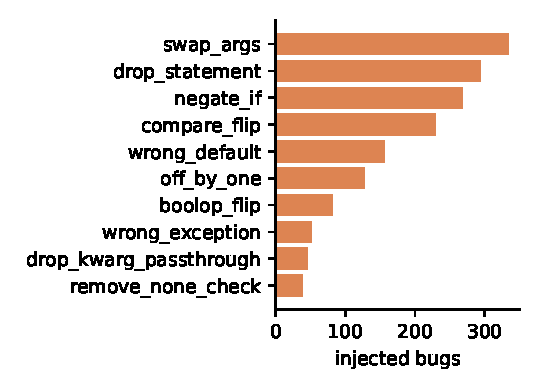
\includegraphics[width=0.45\linewidth]{figs/b5_kinds.pdf}\caption{1{,}628 injected bugs by operator.}\end{figure}
Gemma writes each issue as a user would (public-API reproduction, expected vs actual, 40\% with a traceback,
never naming the internal function). Because real issues mention their target with some rate $\rho_\text{real}$,
synthetic issues are subsampled so that the mention rate matches: keeping all $U$ non-mentioning issues and
$k=\frac{\rho_\text{real}}{1-\rho_\text{real}}U$ mentioning ones gives $\frac{k}{U+k}=\rho_\text{real}$. The distribution check
(\code{src/retrieval/run\_synth\_check.py}) retrains the ranker on real+synthetic data without embedding features
and compares with real-only training on each held-out real repository; it decides Gate B. Issue generation is
running (about 20\,s per issue on the local server).

%==========================================================================================
\section{The reinforcement-learning traverser (designed, data-gated)}
\subsection{MDP}
An episode is one task. The state $s_h=(q,F_h,M_h)$ holds the issue features $q$, the frontier $F_h$ of visited
nodes with their feature vectors (shared with R3), and the marked set $M_h$. Actions are
$\textsc{Expand}(v,\text{dir})$ for $v\in F_h$ and $\text{dir}\in\{\text{out},\text{in}\}$ (the graph has one edge type; we also
distinguish containment), $\textsc{Mark}(v)$ and $\textsc{Stop}$; horizon $H\approx20$. The initial frontier is the seed set
$S$ or BM25's top-$k$. The terminal reward favours recall,
\[
R=F_\beta(M_H,T)-\lambda H,\qquad F_\beta=\frac{(1+\beta^2)PR}{\beta^2P+R},\ \beta>1,
\]
optionally with potential-based shaping $r_h+\gamma\Phi(s_{h+1})-\Phi(s_h)$, $\Phi(s)=-\min_{v\in F,u\in T}d(v,u)$, which
provably leaves the optimal policy unchanged.
\subsection{Policy and learning}
A pointer-style policy scores every candidate action with one shared network over
$[\phi(q)\Vert\phi(v)\Vert e_\text{dir}]$, so a variable-size frontier needs no fixed action dimension:
\[
\pi_\theta(a\mid s)=\frac{\exp f_\theta(a,s)}{\sum_{a'\in\mathcal A(s)}\exp f_\theta(a',s)}.
\]
\emph{Behaviour cloning} on shortest seed$\to$target paths (expert actions $a_h^\star$) minimizes
\[
\mathcal L_\text{BC}(\theta)=-\sum_h\log\pi_\theta(a_h^\star\mid s_h).
\]
\emph{REINFORCE} with a learned baseline $b_\psi$ then follows
\[
\nabla_\theta J(\theta)=\E_{\tau\sim\pi_\theta}\Big[\sum_h\nabla_\theta\log\pi_\theta(a_h\mid s_h)\,\big(G_h-b_\psi(s_h)\big)\Big],\qquad G_h=\sum_{h'\ge h}r_{h'},
\]
and PPO's clipped surrogate is used only if variance is a problem:
\[
J_\text{PPO}(\theta)=\E\big[\min\big(\rho_h\hat A_h,\ \text{clip}(\rho_h,1-\epsilon,1+\epsilon)\hat A_h\big)\big],\qquad \rho_h=\frac{\pi_\theta(a_h\mid s_h)}{\pi_{\theta_\text{old}}(a_h\mid s_h)}.
\]
\emph{Intuition:} BC teaches the policy to walk towards the answer the way a shortest path would; policy
gradients then optimize the actual objective (recall of the final marked set under a step cost), letting the
policy learn when to stop and when exploring a neighbour is worth a step.

\subsection{Why it is gated, and how it would ship}
RL must beat the best non-RL retriever on held-out repositories; with three real training repositories even the
supervised ranker does not beat BM25, so RL waits for the synthetic/external data. Deployment (Option A,
\code{reports/optionAB.md}): a pure-Python policy with JSON weights inside \code{locate.py}, building its graph from
\code{/workspace} with our builder (the organizers' graphs are not reachable from the sandbox).

%==========================================================================================
\section{Lessons learned}
\begin{itemize}
\item \textbf{Measure the harness, not your assumptions.} The test-patch trap, malformed tool calls and context compaction were all invisible until we read raw logs and captured requests.
\item \textbf{Small evaluation sets lie.} On 30 tasks, $\pm$2.5 tasks is one standard error; the protocol now requires 107 tasks, multiple runs and paired tests.
\item \textbf{Time is a first-class metric.} Thinking budget, tool budget and per-task time interact; the fastest configuration with equal accuracy (C6a) is the safest under a 12-hour cap.
\item \textbf{Prompt formatting is part of the model interface.} Markdown in instructions leaked into structured tool calls.
\item \textbf{Learned components need diverse data.} Three repositories are not enough to beat BM25; mined and synthetic data are prerequisites, not extras.
\item \textbf{Shared infrastructure needs defensive engineering}: uneven pipeline splits, per-rank memory budgets, port collisions with other users' services, and self-matching \code{pkill} patterns all cost real time.
\end{itemize}

\section{Status and next steps}
\begin{table}[H]\centering\small
\begin{tabularx}{\linewidth}{lX}\toprule
Done & Data audit; local harness (107 valid); serving; Kaggle pipeline with capture; B1; B2; locator skill; C1--C6; freeze of C6a; rules; LoRA smoke (local); scoreboard; E0 formatting; B4 mining; graph builder; B5 injection; Option A/B memo. \\
Running / queued & Kaggle: LoRA smoke, C6a$\times$4, B0$\times$2 (reference measurement and first SFT data); synthetic issue generation. \\
Next & P5 triage of stochastic tasks (decides whether localization matters for the competition); B5 distribution check (Gate B); E1 rejection-sampling SFT on captured successes + mined tasks, LORO, on rented 80\,GB GPU; E2 expert iteration; C6a submission. \\
Risks & Kaggle GPU availability; QAT+LoRA quality; 12-hour runtime if the scorer runs tasks serially; synthetic-issue distribution shift. \\\bottomrule
\end{tabularx}\end{table}

\appendix
\section{Where things are}
\begin{table}[H]\centering\small
\begin{tabularx}{\linewidth}{lX}\toprule
\code{src/dataio/} & loaders, audit\\
\code{src/groundtruth/map\_patch.py} & B1 patch$\to$node labels\\
\code{src/retrieval/} & text/anchors, context (BM25, graph index), features, baselines, synthetic check\\
\code{src/eval/} & harness patches, gold/empty verification, valid set, scorer-faithful runner, triage, scoreboard, locator evaluation, validator\\
\code{src/sft/} & smoke adapter, capture proxy, exact-format rendering, dataset builder\\
\code{src/mining/}, \code{src/synth/}, \code{src/graphbuild/} & B4 mining, B5 injection and issues, graph builder\\
\code{submissions/} & B0, C1--C6 scaffolds, LoRA smoke\\
\code{scripts/} & serving (\code{start\_server.sh}, patches), local eval, Kaggle kernels/queue, packaging\\
\code{reports/} & all result tables, memos, this report\\\bottomrule
\end{tabularx}\end{table}

\section{Reproducing the main results}
\begin{lstlisting}
.venv/bin/python -m src.dataio.audit                      # data audit
.venv-eval/bin/python -m src.eval.verify_gold --mode gold  # + --mode empty; then src.eval.valid_set
.venv/bin/python -m src.groundtruth.map_patch             # B1
.venv/bin/python -m src.retrieval.run_baselines --seeds 3 # B2 table
.venv/bin/python -m src.eval.eval_locate_skill            # locator skill accuracy
scripts/start_server.sh                                    # local model server (port 8011)
.venv/bin/python scripts/kaggle_eval/make_kernel.py --submission submissions/c6a --run NAME --n 30 --push
.venv/bin/python -m src.eval.triage results/kaggle/NAME/results/NAME
.venv-harness/bin/python -m src.sft.format --roundtrip results/capture.jsonl --trace <trace> --scaffold c6a
\end{lstlisting}

\end{document}
